
\subsection{Linux}

\lstset{language=make}

Before using Hermes2D, you need to make sure that the following packages are installed
on your system:

\begin{center}
\begin{tabular}{ll}
  UMFPACK & \url{http://www.cise.ufl.edu/research/sparse/umfpack/} \\
  FreeGLUT & \url{http://freeglut.sourceforge.net} \\
  Judy & \url{http://judy.sourceforge.net}
\end{tabular}
\end{center}

UMFPACK is the default sparse linear system solver for Hermes2D,
freeglut is  used for visualization and Judy is a sparse array library
used internally by Hermes2D. Please refer to the web pages of these projects for
instructions on how to download and install them. Alternatively, you may want to
consult your system's package manager to have these packages
installed automatically for you. For example, on Debian and Ubuntu systems, you
can install the packages with the command
\begin{lstlisting}
sudo apt-get install libsuitesparse-dev freeglut3-dev libjudy-dev
\end{lstlisting}
% TODO: verify the above
% TODO: mention that we need a recent UMFPACK version, at least 5.1

After downloading \verb"hermes2d-X.Y.Z.tar.bz2" to your home directory, unpack it with
the command
\begin{lstlisting}
 tar xjvf hermes2d-X.Y.Z.tar.bz2
\end{lstlisting}

Go to the unpacked directory, edit the file \verb"Make.config.example" and
follow the instructions therein. In particular, select which compiler to use ({\tt
gcc} or {\tt icc}) and specify the UMFPACK installation directory. When done,
save the file as {\tt Make.config} and type {\tt make}. This should
produce the following files in {\tt hermes2d/lib}:
{\small\begin{verbatim}
   libhermes2d-gcc-g-real.a
   libhermes2d-gcc-O-real.a
   libhermes2d-gcc-g-cplx.a
   libhermes2d-gcc-O-cplx.a
\end{verbatim}}
These are different versions of the library, depending on whether it is a debugging
or optimized ({\tt g} or {\tt O}) and real or complex build.

You may also use one of the predefined files, such as {\tt Make.config.Debian},
in the following way:
\begin{lstlisting}
 cd hermes2d-X.Y.Z
 cp Make.config.Debian Make.config
 make
\end{lstlisting}

Examples from this manual are located in the directory {\tt hermes2d/examples} and
should build with the rest of the library after typing {\tt make}.

For creating your own projects, we suggest the following scheme. Create a directory,
say \verb"~/projects", containing subdirectories with your projects. In the
{\tt projects} directory, create a file named {\tt Make.config} with the following
contents:
\begin{lstlisting}
 HERMES = /home/jakub/hermes2d # replace with your own directory
 include $(HERMES)/Make.config
\end{lstlisting}
In each project subdirectory, use the following {\tt Makefile}:
\begin{lstlisting}
 include ../Make.config
 NAME = name-of-executable
 SRCS = main.cpp
 HLIB = $(HERMES)/lib/libhermes2d-$(CC)-O-real.a
 FLAGS = $(OPT)
 #FLAGS = -ggdb  # for debugging
 include ../Make.common
\end{lstlisting}
The file {\tt Make.common} may contain rules used by all projects:
\begin{lstlisting}
 OBJS = $(SRCS:.cpp=.o)
 $(NAME): $(OBJS) $(HLIB)
       $(CC) $(OBJS) -o $@ $(HLIB) $(LIBS) -pthread
 %.o: %.cpp $(HLIB)
       $(CC) $(FLAGS) -I$(HERMES)/include $(INCLUDES) -c $< -o $@
\end{lstlisting}

% clean:
%         rm -f $(NAME) *.o


%%%%%%%%%%%%%%%%%%%%%%%%%%%%%%%%%%%%%%%%%%%%%%%%%%%%%%%%%%%%%%%%%%%%%%%%%%%%%%%%%%%%%%%%%%%%%%%%%%%%

\subsection{Windows XP/2000}

Download and install the free Dev-C++ IDE from \url{www.bloodshed.net/dev/}
It only has 9 MB and contains a user-friendly IDE and the complete GCC compiler
for Windows called MinGW. When prompted for the installation directory,
use \verb"C:\Dev-Cpp"

To ensure that important files such as the GCC compiler and the libraries can
always be found, right-click My Computer and go to Properties / Advanced / Environment Variables.
Press the New button and enter a variable called ``Path'' containing the
text
\begin{lstlisting}
C:\Dev-Cpp\bin;C:\Dev-Cpp\include;C:\Dev-Cpp\lib
\end{lstlisting}
as shown in Figure \ref{fig:win-env}.

\begin{figure}[ht]
  \medskip \centering
  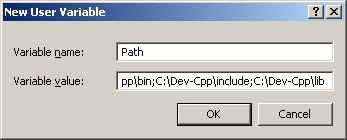
\includegraphics[width=0.53\textwidth]{img/win-env.png}
  \caption{New environment variable dialog box.}
  \label{fig:win-env}
\end{figure}

Since the compilation of libraries that Hermes2D depends on is extremely painful on Windows,
we have prepared a pre-compiled package containing the libraries FreeGLUT, Judy, pthread,
BLAS and UMFPACK. All you have to do is download the file {\tt hermes2d-win32-libs.zip}
from the Hermes2D web page and extract it into \verb"C:\Dev-Cpp". It is crucial that the library
files ({\tt *.a}, {\tt *.dll}) are extracted to the (already existing) directory
\verb"C:\Dev-Cpp\lib" and the header files to \verb"C:\Dev-Cpp\include".

Now download and extract the Hermes2D source archive or check out the latest version with SVN.
Open the file {\tt hermes2d-real.dev}, which is a Dev-C++ project for the real version of Hermes2D
and build the library by pressing Ctrl+F9. Close the IDE and repeat for the complex version
by opening {\tt hermes2d-cplx.dev}

Each example in the {\tt examples/} directory has its own {\tt .dev} file. Open one of them with
Dev-C++ and press F9 to compile and run the example.

As of now it is not possible to compile Hermes2D with the Microsoft compiler. However, it should
be possible to compile your project (or the examples) with MSVC and link with the MinGW libraries.

\newpage
